% Available-capacity replay snippet -- capacities evaluated: 32, 64, 128. cap256 NOT run; do not cite this figure as covering cap256.
% This is a capacity-explicit companion figure, not Figure 2 / Figure 3.
\begin{figure}[t]
  \centering
  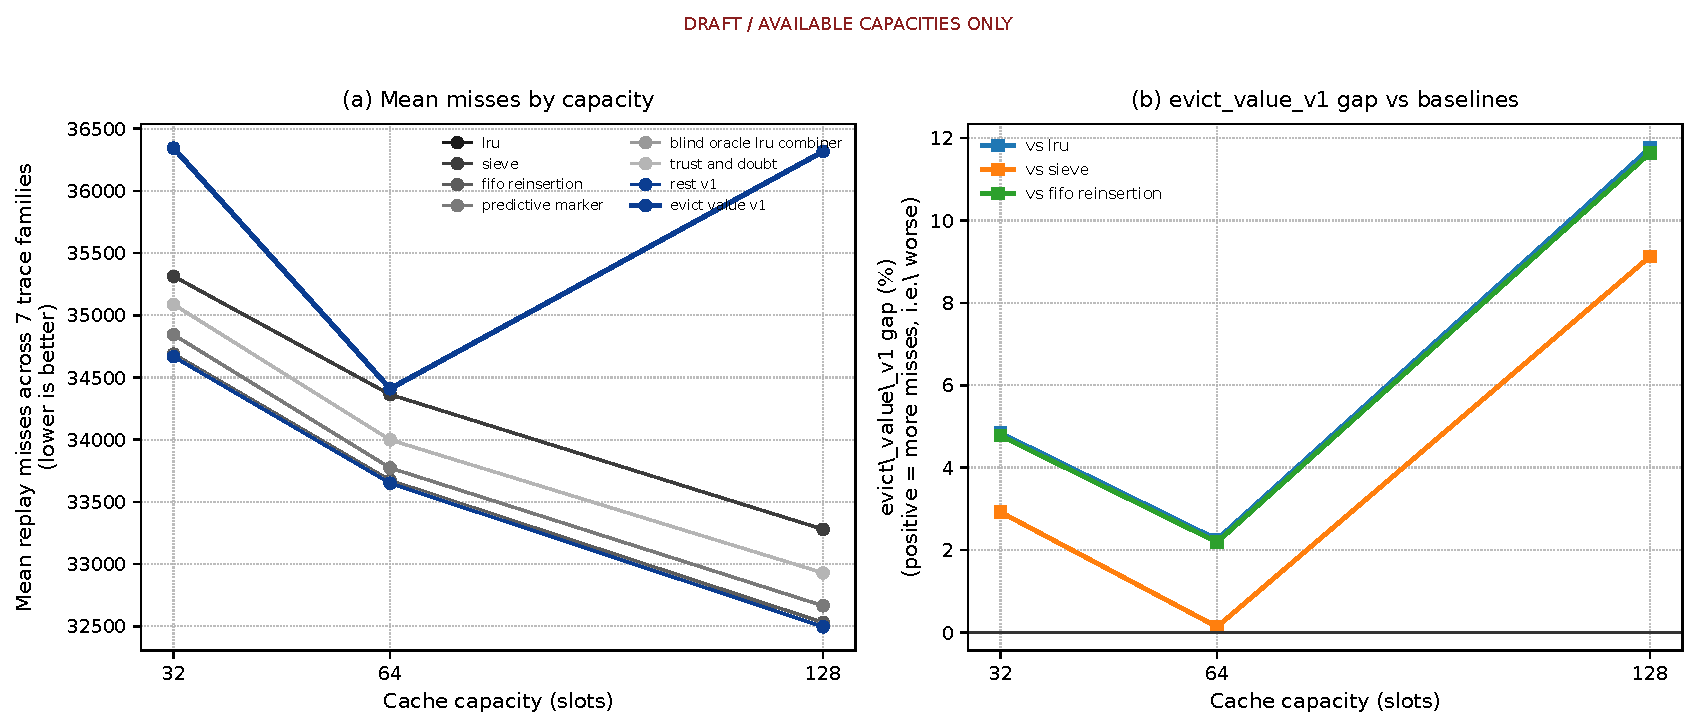
\includegraphics[width=\linewidth]{figures/manuscript/figure_available_capacities_trend.pdf}
  \caption{Capacity-trend comparison across the available-capacity replay (capacities 32, 64, and 128; cap256 not evaluated in this revision). (a) Mean replay misses per policy at each capacity, averaged across the 7 trace families. (b) \texttt{evict\_value\_v1}'s relative miss gap against LRU, SIEVE, and FIFO-Reinsertion at each capacity; positive values indicate more misses than the baseline. The LRU and FIFO-Reinsertion gap curves nearly coincide because the two baselines have nearly identical miss counts in the averaged replay; distinct line styles and markers are used to keep them visually separable. The non-monotonic widening at capacity 128 is discussed in the Limitations section.}
  \label{fig:available-capacities-trend}
\end{figure}
